\documentclass{article}

% - style template
\usepackage{base}

% - title, author, etc.
\title{PHYS4004 - Assignment 4 - Workflow}
\author{Tom Ross - 1834 2884}
\date{\today}

% - headers
\pagestyle{fancy}
\fancyhf{}
\rhead{\theauthor}
\chead{}
\lhead{\thetitle}
\rfoot{\thepage}
\cfoot{}
\lfoot{}

% - document
\begin{document}

The entire code repository can be found at
\url{https://github.com/dgsaf/hpc-assignment-4}.

\tableofcontents

\listoffigures

\listoftables

\clearpage

\section{Interpretation}
\label{sec:interpretation}

\lstinputlisting[
label={lst:count}
, caption={
  The process \lstinline{process count} in \lilf{nextflow/main.nf}.
}
, language=
, morekeywords={process, input, output, container, shell, from, into}
, linerange={48-69}
, firstnumber=48
]{../nextflow/main.nf}

\clearpage

\section{Development}
\label{sec:development}

\lstinputlisting[
label={lst:count}
, caption={
  The channel \lstinline{counted_ch} is duplicated, with one for each of
  \lstinline{process plot_for}, and \lstinline{process plot_xargs}, in
  \lilf{nextflow/main.nf}.
}
, language=
, morekeywords={process, input, output, container, shell, from, into}
, linerange={72-72}
, firstnumber=72
]{../nextflow/main.nf}

\subsection{Bash For Loop}
\label{sec:bash-for-loop}

\lstinputlisting[
label={lst:count}
, caption={
  The process \lstinline{process plot_for} in \lilf{nextflow/main.nf}.
}
, language=
, morekeywords={process, input, output, container, shell, from, into}
, linerange={75-93}
, firstnumber=75
]{../nextflow/main.nf}

\subsection{xargs Command}
\label{sec:xargs-command}

\lstinputlisting[
label={lst:count}
, caption={
  The process \lstinline{process plot_for} in \lilf{nextflow/main.nf}.
}
, language=
, morekeywords={process, input, output, container, shell, from, into}
, linerange={96-113}
, firstnumber=96
]{../nextflow/main.nf}

\section{Execution}
\label{sec:execution}

\subsection{SNR Plot}
\label{sec:snr-plot}

\begin{figure}[h]
  \centering
  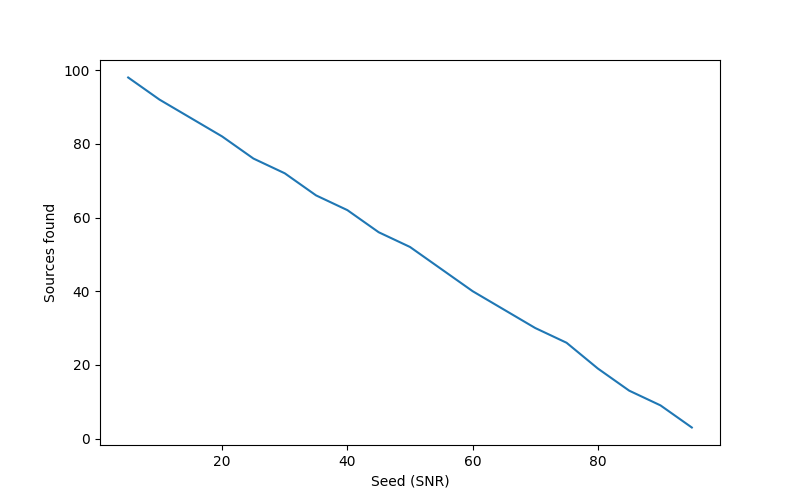
\includegraphics[scale = 0.75]{../nextflow/output/plot_for_1.png}
  \caption[SNR Plot]{
    The Signal-to-Noise Ratio (SNR) is presented for a range of seed SNR values.
    This figure was produced by
    \lstinline[morekeywords={process}]{process plot_for}, for the case of
    \lstinline{cores = 1}.
    No difference was observed between this plot and any of the other plots
    produced for any value of \lstinline{cores}, nor whether if
    \lstinline[morekeywords={process}]{process plot_for} or if
    \lstinline[morekeywords={process}]{process plot_xargs} were used.
  }
  \label{fig:snr-plot}
\end{figure}


\subsection{Workflow DAG}
\label{sec:workflow-dag}

\begin{figure}[h]
  \centering
  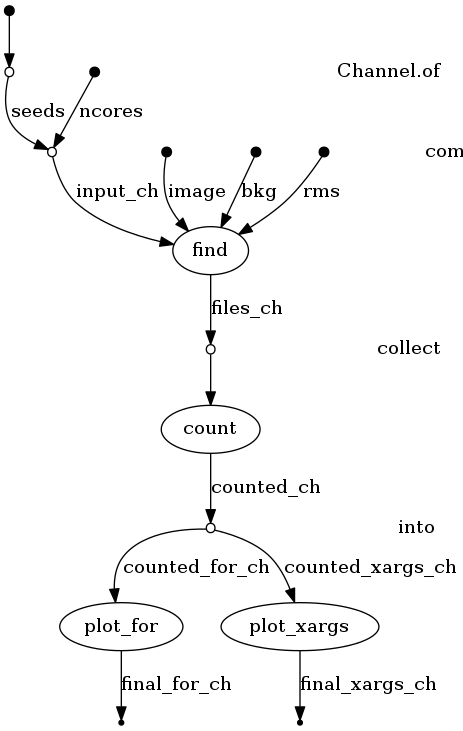
\includegraphics[scale = 0.4]{../nextflow/logs/final_dag.png}
  \caption[Workflow DAG]{
    The Directed Acyclic Graph (DAG) of the workflow is presented.
    Note that the \lstinline{combine} operator (below \lstinline{Channel.of})
    appears to have been cropped out by the tool producing the DAG.
  }
  \label{fig:workflow-dag}
\end{figure}

\clearpage

\section{Analysis}
\label{sec:analysis}

\end{document}
